\section{Zerstörungsfreie Analyse chemischer Zusammensetzungen}\label{sec:materialanalyse}
In diesem Versuchsteil werden mit einem Röntgenenergiedetektor die Fluoreszenz-Spektren von vier verschiedenen unbekannten Legierungen
und einiger Referenzspektren aufgenommen. Damit lassen sich die einzelnen Komponenten der vier unbekannten Legierungen bestimmen.
Außerdem werden die Massenanteile der einzelnen Komponenten einer dieser unbekannten Legierungen bestimmt.\par
Das aufgenommene Fluoreszenz-Spektrum einer Legierung entsteht dadurch, dass die mit der Röntgenröhre erzeugte Röntgenstrahlung
Elektronen mit hohen Bindungsenergien aus den Atomen der Legierung herausschlagen kann, sodass diese frei gewordenen Energieniveaus mit
Elektronen aus höheren Schalen wieder aufgefüllt werden können. Durch diesen atomaren Übergang wird dann wieder Röntgenstrahlung
emittiert, was in dem Fluoreszenz-Spektrum resultiert. Da dieses Fluoreszenz-Spektrum Informationen über die atomaren Übergänge
der Legierungs-Atome beinhält, können so Rückschlüsse auf Materialeigenschaften geschlossen werden.
\subsection{Aufbau}\label{subsec:material_aufbau}
Für die Materialanalyse wird die Cu-Röntgenröhre verwendet. Außerdem wird für die Messung der Röntgenenergiedetektor benutzt, welcher anstelle
des Sensorarms mit dem Zählrohr eingebaut wird. Bei einem Röntgenenergiedetektor handelt es sich im Wesentlichen um eine PIN-Photodiode.
Eine PIN-Photodiode ist eine PN-Diode (Zusammensetzung einer p-dotierten und einer n-dotieren Halbleiterschicht), wobei zwischen
p- und n-dotierter Schicht eine intrinsische Halbleiterschicht (kaum bis nur gering dotiert) eingesetzt wird. Die Röntgenphotonen
erzeugen in der intrinsischen Halbleiterschicht Elektron-Loch-Paare, wobei die Elektronen zu der n-dotierten Schicht und die Löcher
zu der p-dotierten Schicht abgezogen werden. Je energiereicher die Röntgenphotonen sind, desto mehr weitere Elektron-Loch-Paare können durch
Stoßprozesse ausgelöst durch das ursprünglich entstandene Elektron-Loch-Paar erzeugt werden. Somit ist der gemessene Strom
proportional zur Energie der einfallenden Röntgenstrahlung. Ein weiterer Bestandteil des Röntgenenergiedetektors ist ein
Vielkanalanalysator, welcher die unterschiedlichen gemessenen Energien einem Kanal zuordnet, sodass schließlich ein Energiespektrum zu
betrachten ist.\par
In die Kollimatoraufnahme wird ein Kollimator mit \SI{1}{\milli \meter} Spaltbreite eingesetzt.
Dann werden die Abstände zwischen Spaltblende des Kollimators und Drehachse sowie zwischen Drehachse und Eintrittsöffnung des Energiedetektors jeweils
auf ca. 5-6 \unit{\cm} eingestellt. Schließlich wird am Röntgengerät der Taster \textit{COUPLED} gedrückt und der Winkel mit dem Dreheinsteller
\textit{Adjust} auf \SI{45}{\degree} eingestellt, sodass das Target bei \SI{45}{\degree} und der Sensor bei \SI{90}{\degree} steht.
Der hier verwendete Versuchsaufbau ist in \cref{fig:aufbau_material} dargestellt.
\begin{figure}[H]
	\centering
	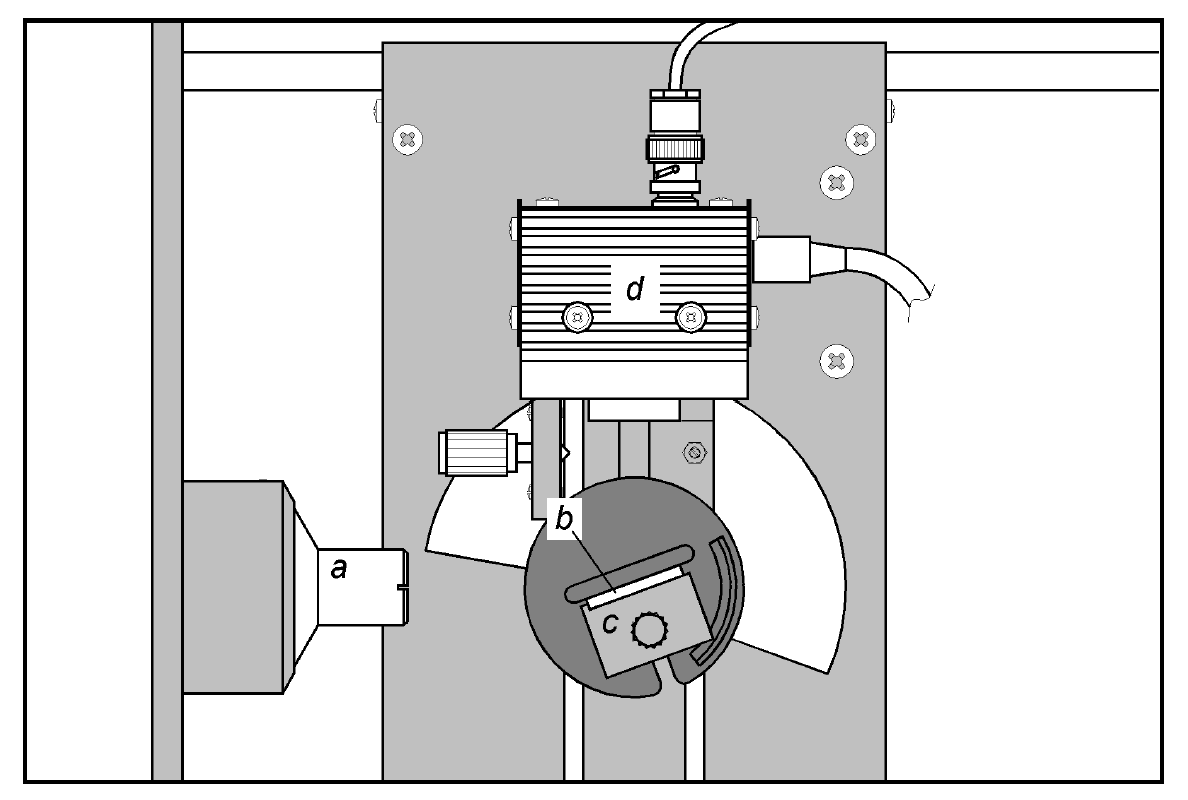
\includegraphics[width=0.6\linewidth]{../figs/aufbau_material.png}
	\caption{Versuchsaufbau zur Materianalyse mit einem Röntgenenergiedetektor:
    a - Kollimator, b - Target, c - Targettisch, d - Röntgenenergiedetektor \cite{material_handblatt}.}
	\label{fig:aufbau_material}
\end{figure}
\subsection{Messung}\label{subsec:material_messung}
Zuerst wird das Kalibriertarget (FeZn-Plättchen) auf den Targettisch gelegt. Zur Aufnahme der Messwerte wird am PC das Programm \textit{Cassy Lab}
verwendet. In \textit{Cassy Lab} wird die Vielkanalmessung mit 512 Kanälen und negativen Pulsen aktiviert. Außerdem wird eine Verstärkung von
\num{-2,5} und eine Messdauer von \SI{180}{\second} eingestellt. Am Röntgengerät wird $U = \SI{35,0}{\kilo \volt}$ und $I = \SI{1,00}{\milli \ampere}$
eingestellt. Dann wird mit dem Schalter HV ON/OFF die Hochspannung eingeschaltet. Dann kann die Spektrumaufnahme am PC gestartet werden.\par
Mit den selben Messparametern werden die Spektren der vier unbekannten Legierungen und die Referenzspektren der Elemente Blei (Pb), Eisen (Fe),
Gold (Au), Indium (In), Kupfer (Cu), Nickel (Ni), Silber (Ag), Titan (Ti), Wolfram (W), Zinn (Su), Zink (Zn) und Zirkonium (Zr) aufgenommen.
\subsection{Auswertung}\label{subsec:material_auswertung}